\documentclass[epsfig]{article}
\usepackage{epsfig}
\usepackage{amsmath}
\usepackage{verbatim}
\usepackage{booktabs}
\usepackage{subfig}
\usepackage{graphicx}
\usepackage{multirow}
\usepackage{epsfig}
\usepackage{amsmath}
\usepackage{graphicx}
\usepackage{subfig}
\usepackage[english]{babel}
\usepackage{rotating}
\usepackage{multirow}
\usepackage[english]{babel}
\textwidth 6.7in
\oddsidemargin -0.1in
\textheight 8.50in
\topmargin -0.55in
\renewcommand{\textfraction}{0.25}
\renewcommand{\floatpagefraction}{0.7}
\begin{document}
\parindent=0pt
\author{Kentaro Hoffman}
\title{COMP/ELEC/STAT 502 HW 05}
\maketitle

  
 \subsection*{Problem 1}
 \begin{table}[htbp] 
\center
\caption{Parameters of Training BP Network to Fit Iris Data Set from the Previous HW}
  \label{tab:NP}
  %\scalebox{0.9}{ % You can scale the size of the table by changing this number
   \scalebox{1.0}{
   \begin{tabular}{p{4cm} p{.05cm} p{8cm}}
\toprule
  \multicolumn{3}{l}{\bf Network parameters} \\
\bottomrule \noalign{\smallskip}
  Topology & & $(1 + 1_{Bias})$ --- $(2 + 1_{Bias})$ --- $1$ \\
  Transfer function & & Hyperbolic Tangent with slope of 1 \\
\toprule
  \multicolumn{3}{l}{\bf Learning parameters} \\
\bottomrule \noalign{\smallskip}
  Initial weights & & drawn from U[-0.1, 0.1] \\
  Learning rate ($\alpha$) & & 0.02\\
  Momentum & & 0.5\\
  Epoch size ($Epoch$)& &  200 \\
  Stopping criteria & &  error ($Err_{train }$) $ \le 0.04 $ OR  learn count (t) $ > 225,000$\\
  Error measure ($Err_{stop}$)& & $ Acc_X = \frac{\# correct\enspace hits}{|X|}\enspace \%$ See formula (2) below \\\toprule
 \multicolumn{3}{l}{\bf Input / output data, representation, scaling} \\
\bottomrule \noalign{\smallskip}
  \# training samples ($N_{tr}$)& & 75 \\
  \# test samples ($N_{tst}$)& & 75 \\
  Scaling of inputs & &  None \\
  Scaling of outputs & &  None \\
%  %\# learn steps performed & & 180,365 (error threshold reached)\\
\toprule
  \multicolumn{3}{l}{\bf Parameters and error measures for performance evaluation} \\
\bottomrule \noalign{\smallskip}
  Error of fit ($Err_{fit}$) & & $ Acc_X = \frac{\# correct\enspace hits}{|X|}\enspace \%$\\
  Final Error of fit for Testing Data &&  0.0267\\
  Final Error of fit for Training Data && 0.000\\
  \# learn steps performed & & 1,725 (threshold for $Err_{stop}$ reached)\\
  Monitoring frequency ($m$) & &  150 learning steps\\
 \bottomrule \noalign{\smallskip}
   \end{tabular}
   } 
\end{table}
 To transition to the Iris dataset, a few modifications were necessary. First was a change in Error measure from mean absolute error to classification accuracy. Specifically, the concept of a correct hit had to be established. Designating an output $y^k$ to be giving the correct response only when $y^k = D^k$ did not lead to any form of convergence. Hence, the following function was applied to the outputs. \\
 \newline
 Let $D_y^k = \min (d_1^k, d_2^k, d_3^k)$. Where $d_1^k$ is the distance from $y^k$ to [1,0,0], $d_2^k$ is from $y^k$ to $[0,1,0]$, and $d_3 ^ k$ is the euclidean distance to $[0,0,1]$, the thresholded output, $\hat{y^k}$ is equal to $[1,0,0]$ if $D_y^k = d_1 ^k$, $[0,1,0]$ if $D_y^k = d_2 ^k$, and $[0,0,1]$ if $D_y^k = d_3 ^k$. Ie it maps every output to the closest possible output. Then when, $\hat{y^k} = D^k$, we would designate this as a correct hit.\\
 \newline
 So in summary, an output is a correct hit if the point that is closest to the output is the desired output. When another possible point is closer, it is an incorrect hit.\\
 \newline
 \section*{Without Cross Validation}
 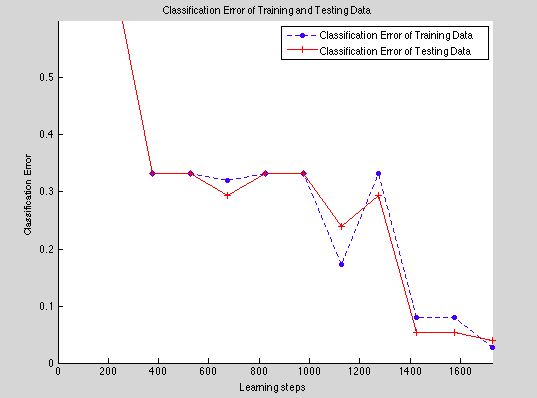
\includegraphics[scale=0.5]{pic1}
 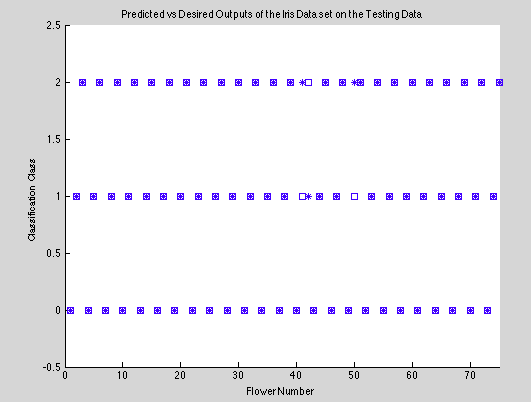
\includegraphics[scale=0.5]{pic2}
 The plots above show the results from the previous homework where no cross validation was applied. The important things to note are how the simulation manages to converge very quickly (1725 steps) and it manages to achieve a respectable 4 percent (3/75) classification error. With k-fold cross validation, if we see that the time till convergence massively increases or if the classification error increases, then it seems likely that the model above is not as useful as it first seems as it has overfitted.
  \begin{table}[htbp] 
\center
\caption{Performance Evaluation for Fold 1}
  \label{tab:NP}
  %\scalebox{0.9}{ % You can scale the size of the table by changing this number
   \scalebox{1.0}{
   \begin{tabular}{p{4cm} p{.05cm} p{8cm}}
\\\toprule
\toprule
  \multicolumn{3}{l}{\bf Parameters and error measures for performance evaluation} \\
\bottomrule \noalign{\smallskip}
  Error of fit ($Err_{fit}$) & & $ Acc_X = \frac{\# correct\enspace hits}{|X|}\enspace \%$\\
  Final Error of fit for Testing Data &&  0.0267\\
  Final Error of fit for Training Data && 0.0400\\
  \# learn steps performed & & 1,725 (threshold for $Err_{stop}$ reached)\\
  Monitoring frequency ($m$) & &  150 learning steps\\
 \bottomrule \noalign{\smallskip}
   \end{tabular}
   } 
\end{table}
\newpage
\section*{Learning History}
\begin{center}
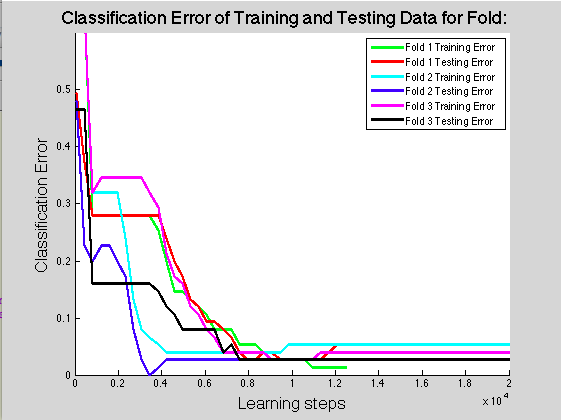
\includegraphics[scale=0.8]{pic3}
\end{center}
Though it may seems convoluted, there are sevearl things that can be noted about the how the ANN is learning. The first is that unlike the previous homework, very few of the folds seem to converge very quickly. They are all downward trending, which means that they are learning the data better, but the fact that 4 out of the 6 (Fold 2 Train, Fold 2 Test, Fold 3 Train and Fold 3 Test) do not terminate, ie get a classification error on the training error of less than 0.04 seems to indicate that these parameters are having a hard time generalizing to the other folds. However, this does not mean that this was useless. On the contrary, the code takes much longer to run, but it does seem to provie outputs that produce good accuracy.
\newpage
\textbf{Fold 1}
\begin{center}
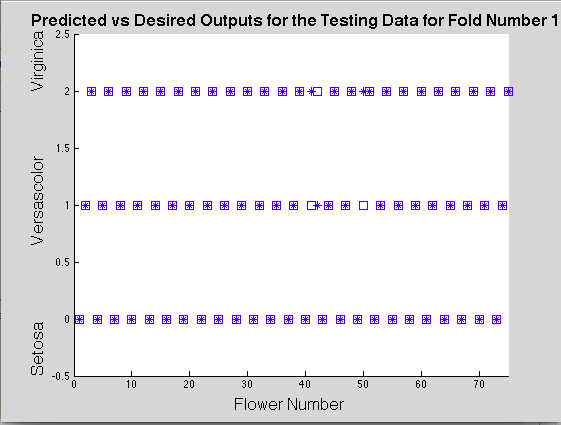
\includegraphics[scale=0.6]{pic4}
\end{center}
 \begin{table}[htbp] 
 

\center
  \label{tab:NP}
  %\scalebox{0.9}{ % You can scale the size of the table by changing this number
   \scalebox{1.0}{
   \begin{tabular}{p{4cm} p{.05cm} p{8cm}}
\\\toprule
\toprule
  \multicolumn{3}{l}{\bf Fold 1 Evaluation} \\
\bottomrule \noalign{\smallskip}
  Final Error of fit for Training Data &&  0.000\\
  Final Error of fit for Testing Data && 0.0400\\
  \# learn steps performed & & 12,750 \\
 \bottomrule {\smallskip}
   \end{tabular}
   } 
\end{table}

\begin{table}[htp]
\caption{Confusion matrices for training and test data for for Fold 1}
\begin{tabular}{c c c}
	(a) Training data, Fold 1 & &
	(b) Test data, Fold 1 \\
% fold 1training
		\begin{tabular} {rrccc}
	&	&	&Predicted Class&	\\
	\multirow{4}{*}{\begin{sideways} True Class \end{sideways}}	&	&Set	&Ver	&Vir	\\
	&Set	&25	&0	&0	\\
	&Ver	&0	&25	&0	\\
	&Vir	&0	&0	&25	\\
	\end{tabular}  & &
% fold 1 test
	\begin{tabular} {rrccc}
	&		&		&Predicted Class&		\\
	\multirow{4}{*}{\begin{sideways} True Class \end{sideways}}	&		&Set	&Ver	&Vir	\\
	&Set	&25		&0		&0		\\
	&Ver	&0		&23		&2		\\
	&Vir	&0		&2		&23		\\
	\end{tabular}  
\end{tabular}  	
\end{table}
From this table, we can see that the although the ANN took much longer to converge, (7600 vs 1725), it was still able to make good predictions, an misclassification of 4 percent (4/75). This is a good sign as it makes it likely that the parameters from the previous homework have not overfitted. Moreover, we can see from the tables that the ANN only has trouble distinguishing between Veriginca and Versacolor, perhaps hinting that Setosa is more different from the other two species. 


\newpage
\textbf{Fold 2}
\begin{center}
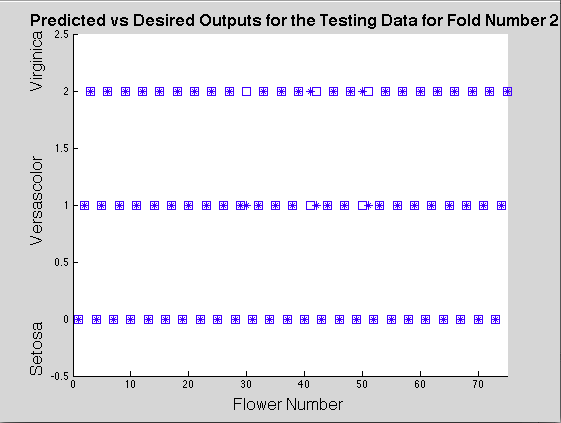
\includegraphics[scale=0.6]{pic5}
\end{center}
 \begin{table}[htbp] 
\center
  \label{tab:NP}
  %\scalebox{0.9}{ % You can scale the size of the table by changing this number
   \scalebox{1.0}{
   \begin{tabular}{p{4cm} p{.05cm} p{8cm}}
\\\toprule
\toprule
  \multicolumn{3}{l}{\bf Fold 2 Evaluation} \\
\bottomrule \noalign{\smallskip}
  Final Error of fit for Testing Data &&  0.0267\\
  Final Error of fit for Training Data && 0.0533\\
  \# learn steps performed & & 225000 (threshold for $Err_{stop}$ reached)\\
 \bottomrule \noalign{\smallskip}
   \end{tabular}
   } 
\end{table}

\begin{table}[htp]
\caption{Confusion matrices for training and test data for for Fold 2}
\begin{tabular}{c c c}
	(a) Training data, Fold 2 & &
	(b) Test data, Fold 2 \\
% fold 1training
		\begin{tabular} {rrccc}
	&	&	&Predicted Class&	\\
	\multirow{4}{*}{\begin{sideways} True Class \end{sideways}}	&	&Set	&Ver	&Vir	\\
	&Set	&25	&0	&0	\\
	&Ver	&0	&25	&0	\\
	&Vir	&0	&0	&25	\\
	\end{tabular}  & &
% fold 1 test
	\begin{tabular} {rrccc}
	&		&		&Predicted Class&		\\
	\multirow{4}{*}{\begin{sideways} True Class \end{sideways}}	&		&Set	&Ver	&Vir	\\
	&Set	&25		&0		&0		\\
	&Ver	&0		&23		&2		\\
	&Vir	&0		&3		&22		\\
	\end{tabular}  
\end{tabular}  	
\end{table}
In terms of accuracy, Fold 2 is a little worse than Fold 1 but not much worse. It misclassifies 5 points insteadof 3 giving it an error of 6.6 percent. In addition the algorithmn never managed to achieve the required error rate so it ran the whoel 225,000 learning steps. In addition, once again, Setosa was not hard to classify, but Versacolor and Virginca gave the algorithmn issues.
\newpage
\textbf{Fold 3}
\begin{center}
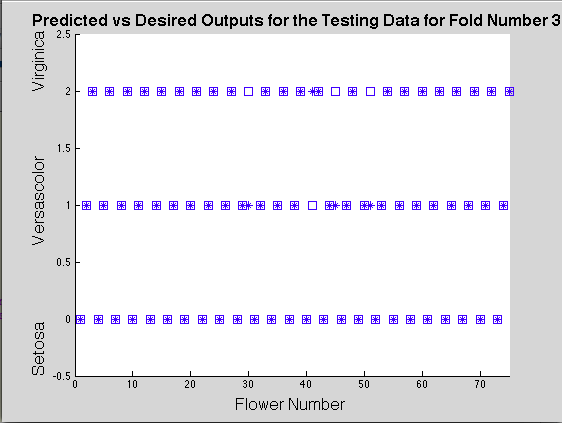
\includegraphics[scale=0.6]{pic6}
\end{center}
 \begin{table}[htbp] 
\center
  \label{tab:NP}
  %\scalebox{0.9}{ % You can scale the size of the table by changing this number
   \scalebox{1.0}{
   \begin{tabular}{p{4cm} p{.05cm} p{8cm}}
\\\toprule
\toprule
  \multicolumn{3}{l}{\bf Fold 3 Evaluation} \\
\bottomrule \noalign{\smallskip}
  Final Error of fit for Testing Data &&  0.0267\\
  Final Error of fit for Training Data && 0.0267\\
  \# learn steps performed & & 225000 (threshold for $Err_{stop}$ reached)\\
 \bottomrule \noalign{\smallskip}
   \end{tabular}
   } 
\end{table}



	\begin{tabular}{c c c}
% blank line for separation
	&  \\
% training confusion matrix:
% captions
	(a) Training data, Fold 3 & &
	(b) Test data, Fold 3 \\
% fold 1training
		\begin{tabular} {rrccc}
	&	&	&Predicted Class&	\\
	\multirow{4}{*}{\begin{sideways} True Class \end{sideways}}	&	&Set	&Ver	&Vir	\\
	&Set	&25	&0	&0	\\
	&Ver	&0	&25	&0	\\
	&Vir	&0	&0	&25	\\
	\end{tabular}  & &
% fold 1 test
	\begin{tabular} {rrccc}
	&		&		&Predicted Class&		\\
	\multirow{4}{*}{\begin{sideways} True Class \end{sideways}}	&		&Set	&Ver	&Vir	\\
	&Set	&25		&0		&0		\\
	&Ver	&0		&24		&1		\\
	&Vir	&0		&3		&22		\\
	\end{tabular}  
\end{tabular}  \\
In Fold 3, things are similar to how they were in Fold 2. The ANN was never able to converge, but it managed to give solid accuracies with 2.6 percent (2/75 misclassifcations) on the training and testing data, and 4/75 or a 5 percent error for the original testing data. Once again, the Versacolor and the Virginca were the ones that the algorithmn had a hard time classifying.
\newpage
\section*{Table}
\begin{center}
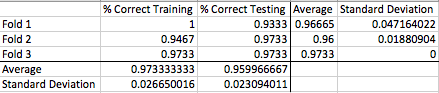
\includegraphics[scale=1]{pic7}
\end{center}
From this table, we get another view at the variations among the Folds and in the folds. The first and perhaps most important thing to note is that all of the Averages were above 95 percent meaning that in all cases, this set of parameters is a yeilds good accurate perdictions. However, the standard deviation illustrates some disturbances. The accuracy between the training and the testing samples can be quite large as Fold 1 has a training accuracy of 1 but a testing accuracy of 0.93. On the other hand Fold 3 has both of the accuricies be 0.97. So perhaps some more folds are needed to give a better image of the accuracy of the dataset. \\
\newline
\textbf{Summary}
In summary, although the runtime of the algorithmn has increased, and the folds have varying levels of accuracy, the high accuracy of the results makes me inclinded to say that this set of parameters has produced generalizable results.
\newpage
\section*{Question 2.1}
\section*{2}
Below are the parameters for the Communication Problem. When multiple parameter values were tried, the optimal is designated with an asterisk.
	\begin{table}[htbp] 
\center
\caption{Parameters of Training BP Network to Fit Question 2.1}
  \label{tab:NP}
  %\scalebox{0.9}{ % You can scale the size of the table by changing this number
   \scalebox{1.0}{
   \begin{tabular}{p{4cm} p{.05cm} p{8cm}}
\toprule
  \multicolumn{3}{l}{\bf Network parameters} \\
\bottomrule \noalign{\smallskip}
  Topology & & $(1 + 1_{Bias})$ --- $(3^*/10/20 + 1_{Bias})$ --- $1$ \\
  Transfer function & & Hyperbolic Tangent with slope of 1 \\
\toprule
  \multicolumn{3}{l}{\bf Learning parameters} \\
\bottomrule \noalign{\smallskip}
  Initial weights & & drawn from U[-0.1, 0.1] \\
  Learning rate ($\alpha$) & & 0.1/0.01*/0.001/0.0001\\
  Momentum & & 0/0.8/1\\
  Epoch size ($Epoch$)& &  100 \\
  Stopping criteria & &  error ($Err_{stop}$) $ \le 0.01 $ OR  learn count (t) $ > 300,000 $\\
  Error measure ($Err_{stop}$)& & MSE of the unscaled training data see formula (1) below\\\toprule
 \multicolumn{3}{l}{\bf Input / output data, representation, scaling} \\
\bottomrule \noalign{\smallskip}
  \# training samples ($N_{tr}$)& & 100 \\
  Scaling of inputs & &  Inputs were divided by 2.1 so that they can span from [-0.95, 0.95] \\
  Scaling of outputs & &  maps raw inputs to [-0.5,0.5] \\
%  %\# learn steps performed & & 180,365 (error threshold reached)\\
\toprule
  \multicolumn{3}{l}{\bf Parameters and error measures for performance evaluation} \\
\bottomrule \noalign{\smallskip}
  Error of fit ($Err_{fit}$) & & Same as Error Measure\\
  Final Error of fit for Training Data && 0.0100\\
  \# learn steps performed & & 79,800 (threshold for $Err_{stop}$ reached)\\
 \bottomrule \noalign{\smallskip}
  \end{tabular}
   } % end scalebox
\end{table}
\textbf{Stopping Criteria}\\
(1) $ Err_{stop} = {1\over{N_{tr}}}\sum_{k=1}^{N_{tr}} (D^k-y^k)^2$\label{err-stop}, where $D^k$ is the unscaled output for the kth  pattern, $y^k$ is the unscaled output of the simulation for the kth  pattern, $N_{tr}$ is the number of training samples.\\
\textbf{Best Results}
\begin{center}
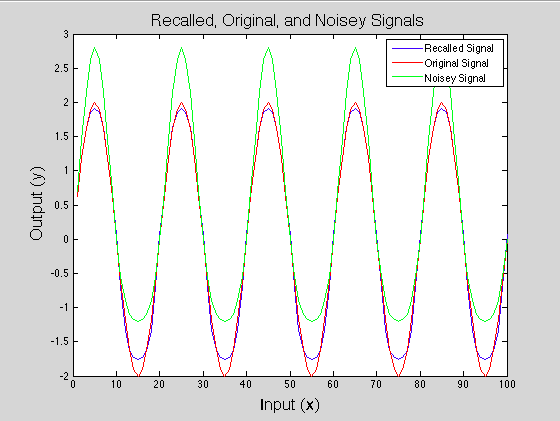
\includegraphics[scale=0.38]{pic8}
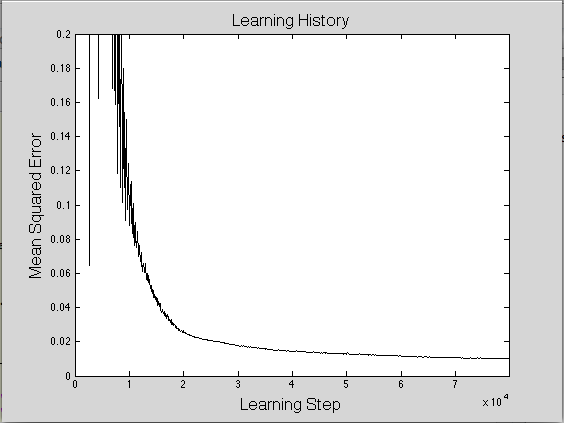
\includegraphics[scale=0.38]{pic9}
\end{center}
From the plots above, we can see that the ANN has done an fairly well job of learning the pattern. The plot on the left shows that while the ANN was able to reduce a substantial amount of the noise that was added to the system. However some issues remain at the peaks of the sine waves. Moreover, the learning History of the ANN was very smooth and shows that the learning process also had no major difficulties.

\section*{Number of Perceptrons}
\begin{center}
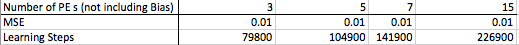
\includegraphics[scale=0.9]{pic10}
\end{center}
In each of the following experiments, the number of PE were varied between 3 and 20.
\newline
\begin{center}
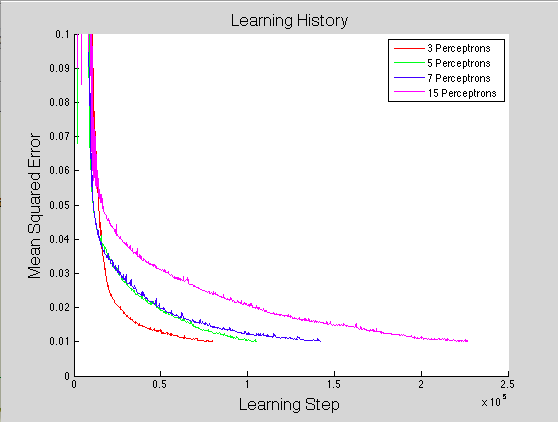
\includegraphics[scale=0.7]{pic11}
\end{center}
From the learning history, we can deduce a very clear pattern. Varying the number of perceptrons seems to make the ANN take longer to converge. This effect seems to be working in an ordered fashion as well because 5 took longer than 3, 7 took longer than 5 and 15 took longer than 7. This accords with my study of Perceptrons in the previous HW where it seemed that as long as there are enough perceptrons so that the Network can converge (usually more than 1 or 2), then the fewest number of perceptrons is desireable. This is most likely due to the fact that a network with more perceptrons is more complex and would thus require more time for it to learn the same data. So 3 will the be number of perferred perceptrons for this question.\\
 
(The plot of Desired vs Output is omitted as all the perceptrons converge to the same MSE so they have the same Output plot as the one seen above).

\section*{Learning Rate}
\begin{center}
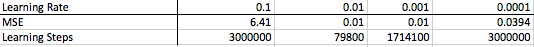
\includegraphics[scale=1]{pic12}
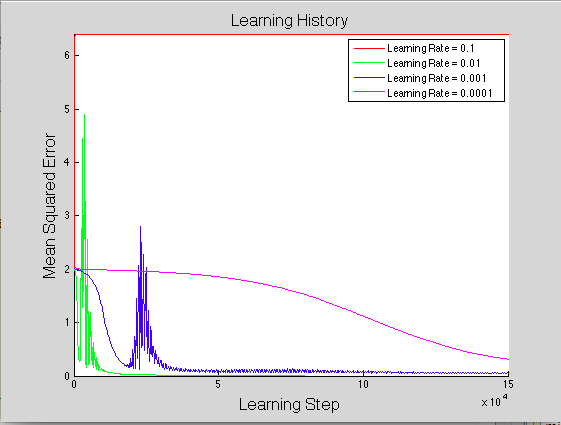
\includegraphics[scale=0.42]{pic13}
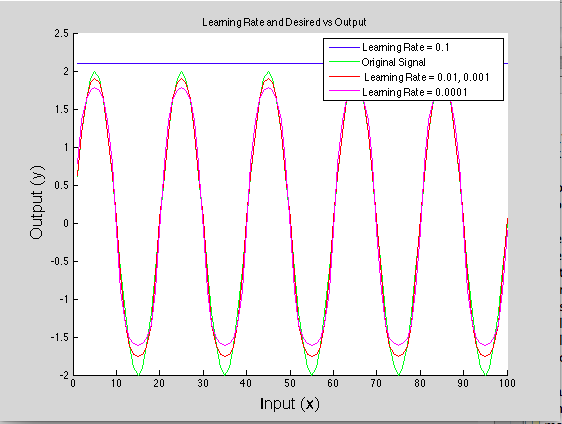
\includegraphics[scale=0.42]{pic14}
\end{center}
From the plot, we can see that like the number of perceptrons, the learning rate is no good when it is too large (0.1) or when it is too small (0.0001). When the learning rate is too large, as you can see on the Desired vs Output graph, the outputs will start to converge to a completely different value than the desired values. However, if the values are too small, as seen in the learning history plot above, it takes longer and longer for the ANN to converge. So the optimal ANN in this case would be 0.01.

\newpage
\section*{Question 2.2}
For the following part of the HW, the following parameters were used:
	\begin{table}[htbp] 
\center
\caption{Parameters of Training BP Network to Fit Question 2.1}
  \label{tab:NP}
  %\scalebox{0.9}{ % You can scale the size of the table by changing this number
   \scalebox{1.0}{
   \begin{tabular}{p{4cm} p{.05cm} p{8cm}}
\toprule
  \multicolumn{3}{l}{\bf Network parameters} \\
\bottomrule \noalign{\smallskip}
  Topology & & $(1 + 1_{Bias})$ --- $(79 + 1_{Bias})$ --- $1$ \\
  Transfer function & & Hyperbolic Tangent with slope of 1 \\
\toprule
  \multicolumn{3}{l}{\bf Learning parameters} \\
\bottomrule \noalign{\smallskip}
  Initial weights & & drawn from U[-0.1, 0.1] \\
  Learning rate ($\alpha$) & & 0.01\\
  Momentum & & 0.8\\
  Epoch size ($Epoch$)& &  100 \\
  Stopping criteria & &  error ($Err_{stop}$) $ \le 0.01 $ OR  learn count (t) $ > 300,000 $\\
  Error measure ($Err_{stop}$)& & MSE of the unscaled training data see formula (1) below\\\toprule
 \multicolumn{3}{l}{\bf Input / output data, representation, scaling} \\
\bottomrule \noalign{\smallskip}
  \# training samples ($N_{tr}$)& & 100 \\
  Scaling of inputs & &  The Inputs of the first signal were divided by 1.9 so that they can span from [-0.95, 0.95] The second set of Inputs were  divided by 4.8 for the same reasons\\
  Scaling of outputs & & Both of the signals were scaled so that they would  maps raw inputs to [-0.5,0.5] \\
%  %\# learn steps performed & & 180,365 (error threshold reached)\\
\toprule
  \end{tabular}
   } % end scalebox
\end{table}

\begin{center}
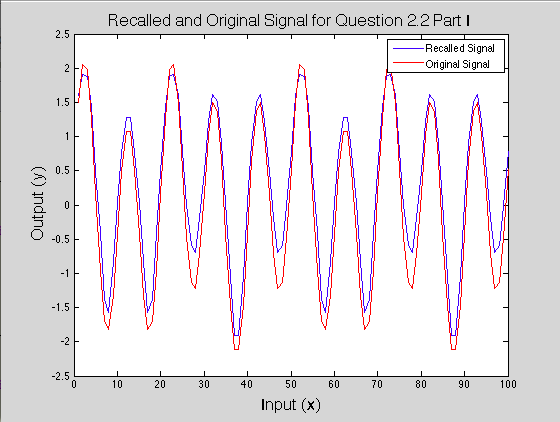
\includegraphics[scale=0.4]{pic15}
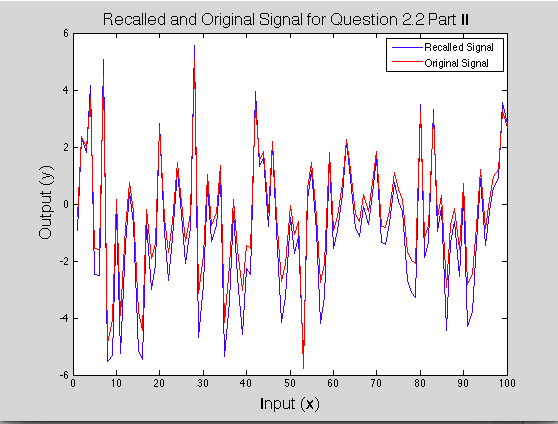
\includegraphics[scale=0.4]{pic16}
\end{center}
From the plots above, we can see that although the two signals have different ranges, and thus require different factors of scaling,  the ANN is doing a good job recovering the original signal. Naturally, it is having difficulties with the more complicated Part II inputs and especially those that have a negative output, but overall, the filtering does give the user a good idea of what the underlying singal looked like.

\end{document}